% Options for packages loaded elsewhere
\PassOptionsToPackage{unicode}{hyperref}
\PassOptionsToPackage{hyphens}{url}
%
\documentclass[
]{article}
\title{Final Project Part 2}
\author{Vincent Zhang}
\date{3/7/2022}

\usepackage{amsmath,amssymb}
\usepackage{lmodern}
\usepackage{iftex}
\ifPDFTeX
  \usepackage[T1]{fontenc}
  \usepackage[utf8]{inputenc}
  \usepackage{textcomp} % provide euro and other symbols
\else % if luatex or xetex
  \usepackage{unicode-math}
  \defaultfontfeatures{Scale=MatchLowercase}
  \defaultfontfeatures[\rmfamily]{Ligatures=TeX,Scale=1}
\fi
% Use upquote if available, for straight quotes in verbatim environments
\IfFileExists{upquote.sty}{\usepackage{upquote}}{}
\IfFileExists{microtype.sty}{% use microtype if available
  \usepackage[]{microtype}
  \UseMicrotypeSet[protrusion]{basicmath} % disable protrusion for tt fonts
}{}
\makeatletter
\@ifundefined{KOMAClassName}{% if non-KOMA class
  \IfFileExists{parskip.sty}{%
    \usepackage{parskip}
  }{% else
    \setlength{\parindent}{0pt}
    \setlength{\parskip}{6pt plus 2pt minus 1pt}}
}{% if KOMA class
  \KOMAoptions{parskip=half}}
\makeatother
\usepackage{xcolor}
\IfFileExists{xurl.sty}{\usepackage{xurl}}{} % add URL line breaks if available
\IfFileExists{bookmark.sty}{\usepackage{bookmark}}{\usepackage{hyperref}}
\hypersetup{
  pdftitle={Final Project Part 2},
  pdfauthor={Vincent Zhang},
  hidelinks,
  pdfcreator={LaTeX via pandoc}}
\urlstyle{same} % disable monospaced font for URLs
\usepackage[margin=1in]{geometry}
\usepackage{graphicx}
\makeatletter
\def\maxwidth{\ifdim\Gin@nat@width>\linewidth\linewidth\else\Gin@nat@width\fi}
\def\maxheight{\ifdim\Gin@nat@height>\textheight\textheight\else\Gin@nat@height\fi}
\makeatother
% Scale images if necessary, so that they will not overflow the page
% margins by default, and it is still possible to overwrite the defaults
% using explicit options in \includegraphics[width, height, ...]{}
\setkeys{Gin}{width=\maxwidth,height=\maxheight,keepaspectratio}
% Set default figure placement to htbp
\makeatletter
\def\fps@figure{htbp}
\makeatother
\setlength{\emergencystretch}{3em} % prevent overfull lines
\providecommand{\tightlist}{%
  \setlength{\itemsep}{0pt}\setlength{\parskip}{0pt}}
\setcounter{secnumdepth}{5}
\usepackage{amsmath}
\usepackage{booktabs}
\usepackage{caption}
\usepackage{longtable}
\ifLuaTeX
  \usepackage{selnolig}  % disable illegal ligatures
\fi

\begin{document}
\maketitle

(Note, this is late, and I used up two 24-hour late extensions already!)

\hypertarget{abstract}{%
\section{Abstract}\label{abstract}}

Is there a significant relationship between the age of a person, and
their COVID-19 vaccine hesitancy? When we look at the pressing world
today, it is perhaps essential to understand what are the underlying
causes for why people are unwilling to get vaccines, if it were our
objective to improve vaccine turnouts. In this paper, I explore more
deeply one of these potential variables: age. Is it the case that
younger people are less likely to be hesitant or more hesitant to
COVID-19 vaccines? Or, do we see that there is no significant evidence
imply such a relationship. Understanding this may allow us to understand
more about why people hesitate to, and thus perhaps also give insight
into what demographics social programs can focus on if they were to try
to improve vaccine acceptance, if it is the case that there is a
relationship.

\hypertarget{description}{%
\section{Description}\label{description}}

The data I chose comes from OpenICPSR, a repository for covid-related
data. A formal citation is included at the end of this document. The
data comes from a COVID-19 Vaccine Hesitancy Survey study that was
conducted and updated from March 2020 to June 2021. Notice that this
survey study includes times before and after vaccine roll outs, as its
original intention is to assess change in attitude towards issues
related to COVID-19, but we will readopt this data for our purposes of
examining the relationship between age and hesitancy. One thing to note
is that this data used Internet-based samples, since it was an opt-in
internet based sampling; the authors admit limitations, stating--on
quote--``This survey used Internet-based samples, which allowed us to
rapidly collect information and to avoid person-to-person contact.
However, internet samples may have inherent biases. There is sampling
bias in that individuals who participate need to have access to the
internet, so individuals of lower socioeconomic status will be less
likely to participate''. This is a limitation in the data collection
that we should take into account in our analysis later. This study was
also surveyed in many different countries, including the United States,
mainland China, Taiwan, Indonesia, India, and Malaysia. These data were
collected in waves (mainly, 4 for Taiwan, Indonesia, Inda, and Malaysia,
but 5 for China and 9 for the United States). This data was collected by
researchers in the schools of medicine, routinely collected in waves,
and funded by funded by organizations such as, National Institute of
Allergy and Infectious Diseases, National Science Foundation, and
Division of Social and Economic Sciences. Furthermore, the ethical
protocol for the conducting of this research project was approved by
committees including University of Michigan Health Sciences and
Behavioral Sciences Institutional Review Board, the Fudan University
School of Public Health ethical review committee, the National Taiwan
University Hospital Research Ethics Committee, the Universiti Tunku
Abdul Rahman, the Institutional Review Board at Universitas Syiah
Kuala/Dr.~Zaionel Abidin Hospita, Indonesia, and the Sigma-IRB in New
Delhi, India. Overall, we can trust that our data was reliably
collected, and thus perform analysis on said data.

One thing to note is that our data includes many waves for six
countries. To make analyzing data more manageable, I have chosen a
subset of this data. Namely, there are four subsets we are concerned
with: 1. the China sample before the vaccine rollout, on the first wave,
which was collected on March 2020. 2. the China sample after the vaccine
rollout, on the last wave to date, which was collcetedd on June 2021. 3.
the US sample before the vaccine rollout, on the first wave, which was
collected on March 2020. 4. the US sample after the vaccine rollout, on
the last wave to date, which was collcetedd on June 2021.

The surveyed data is rather dense with descriptions and information, and
not all will be used for our intended purposes, but here are what some
of the observations in our data is, and what they mean. Note, each of
these observations describe a person's survey response:

\begin{enumerate}
\def\labelenumi{\arabic{enumi}.}
\tightlist
\item
  \textbf{ctry}: the country the sample was taken from (\emph{for our
  purposes, we will be looking at China (CN) and United States (US)})
\item
  \textbf{waveno}: the wave number representing which wave the data was
  collected from (\emph{for our purposes, we will be looking at the
  first and last waves})
\item
  \textbf{d\_age\_yr}: the self-reported age of the participant (how
  many years old), which will be the main focus of our research.
\item
  \textbf{d\_age\_cat}: the self-reported age of the participant, but in
  categories, rather than a specific number
\item
  \textbf{v\_profile} : this is a statistic that is geared towards
  pre-vaccine rollout. This survey data is based on the folowing
  question (I will copy and paste from the code book). Note that, people
  were surveyed with two varying variables, the effectiveness, and how
  safe they are, which are the next two variables in this list:

  \begin{itemize}
  \tightlist
  \item
    A vaccine is currently not available for the new coronavirus strain
    (called SARS-CoV-2 and which causes COVID-19). Imagine that a new
    coronavirus vaccine has just been developed. It has received the
    same testing as the adult influenza vaccine. The government is
    offering it as a free and optional vaccine.
  \item
    Would you accept a coronavirus vaccine which is 95\% effective, with
    a 5\% (or 20\%) chance of a side effect like fever?
  \item
    95\% effective means that there is a 95\% (or 50\%) reduction in
    disease among those vaccinated compared to those unvaccinated.
    6.\textbf{v\_eff} : either 50\% effectivness or 95\% effectiveness
  \end{itemize}
\item
  \textbf{v\_saf} : either 5\% change of side effect, or 20\% change of
  side effect
\item
  \textbf{v} : this is a statistic that is based on the previous
  question (the past 3 stats), in which answer yes if they would take
  the vaccine.
\item
  \textbf{v1\_plan} : this is geared towards post-vaccine rollout. This
  asks, about the participant's vaccination intent by asking how much
  they would agree/disagree with the following statement: ``i plan on
  getting the COVID-19 vaccine''
\item
  \textbf{vaxed} : whether a participant has gotten the vaccine or not.
\item
  \textbf{vax\_hes} : this is a dummy categorical variable (0 or 1), and
  is based on a set of 10 items from Akel (included in the bibliography
  section below), to determine whether a person is in general more
  hesitant than not in getting the vaccine.
\item
  !\textbf{r2\_1} : the participant's perceived risk of death: what do
  they think their risk of dying from covid is on a scale from 1-10?
\item
  !\textbf{r7} : the participant's confidence in scientists in how much
  they know about coronavirus.
\item
  !\textbf{d\_politics}: the policial affiliation of the participant. is
  it the case that younger people are more likely to be a part of one
  affiliation than another? this is a possible confounding variable we
  may want to take into consideration.
\end{enumerate}

These are only a few out of the 58 different variables collected in this
data set. However, I have filtered out, and presented the data that I
think might potentially be useful in our analysis of how age might
contribute to vaccination hesitancy. One thing to notice is that in
numbers 12 to 14, there are exclamation points in the front of the
variables. This is to indicate that I believe these are potential
confounders, which is why I did not exclude them from our list of
relevant data points. For example, young people are probably in less
risk to die, is the fact that they feel less at risk to die a
contributor to them also being less or more hesitant to vaccines? Or,
older people might be more likely to be skeptical about scientists (or
less likely), is this possibly a confounder for why they are more or
less hesitant towards vaccines? Finally, young people are more likely to
be in a particular political affiliation than another, is this a
possible reason for more or less hesitancy towards vaccines because they
are part of that polotical affiliation, and not actually because they
are young? These are questions I want to consider moving forward.

Looking at this data, we also should consider what population this data
is actually representing. According to the researchers, the required
sample size is around 800 for most country at each wave, and we see that
each of our data sets, per wave, reach that threshold. The one exception
is the US March 2020 wave, which only holys 691 observations. The other
dataset waves, have 971, 1070, and 954 samples, in the order of China
June 2021, China March 2020, and US June 2021 in that order. One thing
we might have to note is that these samples are slightly more geared
torwards the young adult population, and does not include as many
elderly as we would like, or younger teens and kids, but other than
that, we would expect that this sample is a solid representation of the
actual population we want to make conclusions or do social science
inquiry on (which is, the Chinese and US population).

\emph{Let us look at how the data is formatted, and how we can make
sense of it:}

The data is split into 30 different .sasb7dat files, 4 waves for each of
the countries India, Indonesia, Malaysia, and Taiwan, 5 waves for China,
and 9 waves for US. To reduce the complexity of all the data we have to
analyze, and I broke it down into four of these files that I think would
give us the most insight, while also limiting the number of confounders
we would have to take into consideration. The four are the four I
mentioned before, but to reiterate, they are China 2020 March, US 2020
March, China 2021 June, and US 2021 June. The reason for choosing two
different countries is to be able to compare the data we found in each
to see if there is anything to sugggest that the patterns we seee in our
data are abstractable to the world in general. The reason for choosing
one before vaccine rollout, and one after vaccine rollout is to see how
people are hesitant in hindsight of the vaccine, but also in pre-sight.
With that being said, I selected the 14 data (columns) I mentioned
previously and filtered out the other 44 variables (columns).

Let us dig more into what our data actually looks like:

Our data is a mixture of characters, describing things in categories
(for this reason, even though these columns are ``characters'', i would
consider this categorical in nature), ordinal numeric representing range
of categories (for instance, in R7 (confidence in scientists), 1
represents not confident, 2 represents somewhat confident, and 3
represents very confident), or numeric ranges scales such as R2\_1
(perceived risk of death), where participants rate on a scale from 0 to
100. Overall, our data is ranging in data types and data
representations, some categorical, some ordinal, some qualitative, etc.
One thing to also note is that depending on whether we are working with
before or after vaccine rollout, there are missing variables (like
v\_eff, v\_saf, and v\_profile, which were questions asked before there
was a vaccine). Or, depending on the countries, different questions are
asked, so the question on political affiliation is not found in the
China data, and the question on perceived risk of death is not found in
the US data. These are things we will need to account for later on.

To detail more into what the data looks like, I have included below the
what the some of the presentable stats from the summary statistic looks
like for China 2021 June:

\begin{enumerate}
\def\labelenumi{\arabic{enumi}.}
\tightlist
\item
  \textbf{ctry}: CN (meaning china)
\item
  \textbf{waveno}: 9 (meaning the 9th wave, or the most recent one)
\item
  \textbf{d\_age\_yr}: mean: 44.63, minimum: 18, maximum: 78 (meaning
  that the average age of the surveyer is 44)
\item
  \textbf{v1\_plan} : mean: 2.124 (1 being strongly agreeing with
  getting the coivd vaccine, and 5 being strongly disagreeing)
\item
  \textbf{vaxed} : mean: 0.892 (meaning 89\% have gotten covid vaccine)
\item
  \textbf{vax\_hes} : mean: 0.229 (meaning 22.9 percent are hesitant)
\item
  \textbf{r2\_1} : mean: 34.67 (meaning on a scale of 100, the average
  person feels lile their risk of death is 34\%)
\item
  \textbf{r7} : mean: 2.688 (1 being not confident, 3 being very
  confident in scientists' knowledge in covid)
\end{enumerate}

\hypertarget{visualization}{%
\section{Visualization}\label{visualization}}

The two variables I will be analzing will be:

\begin{enumerate}
\def\labelenumi{\arabic{enumi}.}
\tightlist
\item
  d\_age\_yr (the self-reported age of the participant in the survey)
\item
  vax\_hes (the hesitancy of the participant in getting a vaccine)
\end{enumerate}

I will be including the statistic for all four of the groups (namely,
China 2021 June, China 2020 March, US 2021 June, US 2020 March):

Here are the means and standard errors of the means for the two
variables in question for the four data sets, and they are
self-explanatory

\captionsetup[table]{labelformat=empty,skip=1pt}
\begin{longtable}{r|rr}
\caption*{
{\large Before Vaccine Rollout} \\ 
{\small March 2020}
} \\ 
\toprule
\multicolumn{1}{l}{} & Mean & Standard Error \\ 
\midrule
China Age & 41.4672897 & 0.45123855 \\ 
China Vax Hes & 0.2293307 & 0.01319569 \\ 
US Age & 47.4413893 & 0.63055310 \\ 
US Vax Hes & 0.3303835 & 0.01807706 \\ 
\bottomrule
\end{longtable}
\captionsetup[table]{labelformat=empty,skip=1pt}
\begin{longtable}{r|rr}
\caption*{
{\large After Vaccine Rollout} \\ 
{\small June 2021}
} \\ 
\toprule
\multicolumn{1}{l}{} & Mean & Standard Error \\ 
\midrule
China Age & 44.6292482 & 0.48803464 \\ 
China Vax Hes & 0.2296601 & 0.01350511 \\ 
US Age & 48.4297694 & 0.57442020 \\ 
US Vax Hes & 0.3779193 & 0.01580622 \\ 
\bottomrule
\end{longtable}

Temporarily, I will only be doing the visualization for one of these
datasets (namely, the US 2021 June dataset), but will consider doing
visualization for all of then in the future if I find to to be useful to
do so.

Below are visualizations of the distribution of our two variables

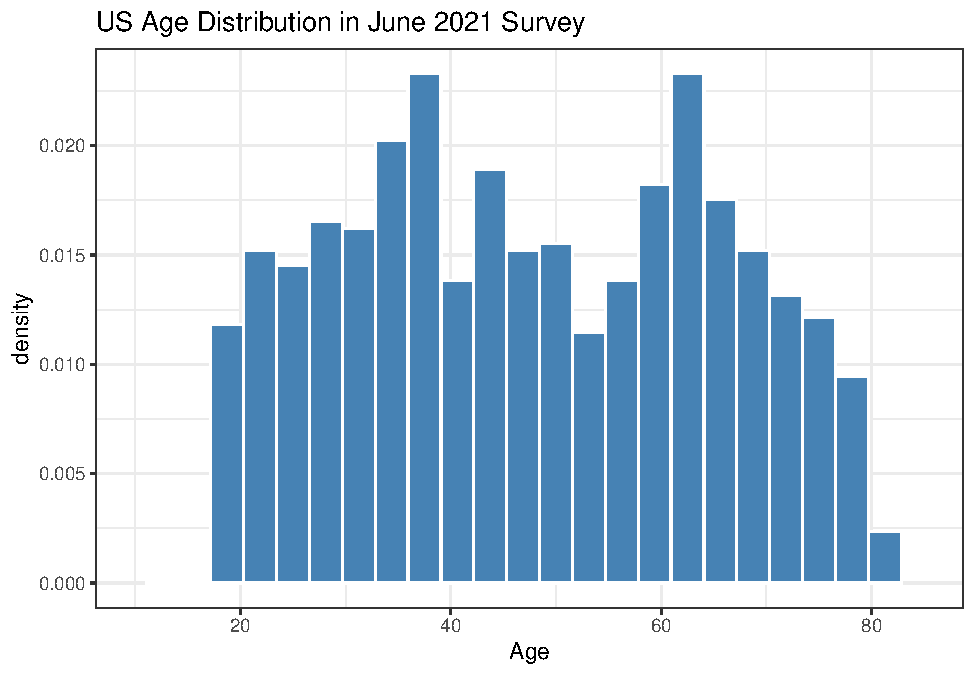
\includegraphics{Untitled_files/figure-latex/unnamed-chunk-3-1.pdf}
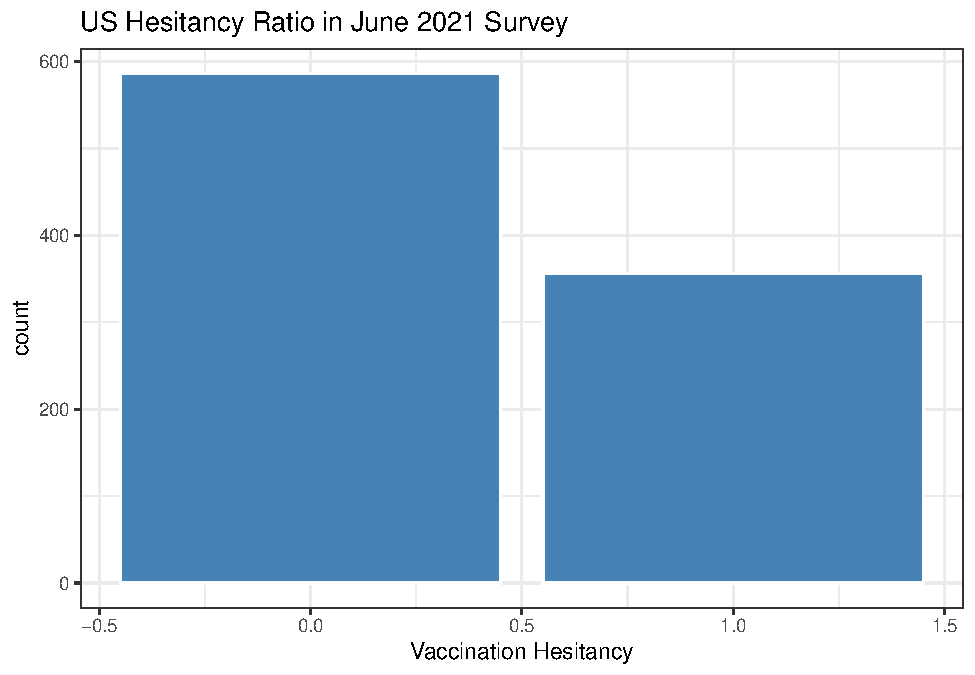
\includegraphics{Untitled_files/figure-latex/unnamed-chunk-3-2.pdf}

Below is a visualization of the distribution of our two variables
plotted against each other

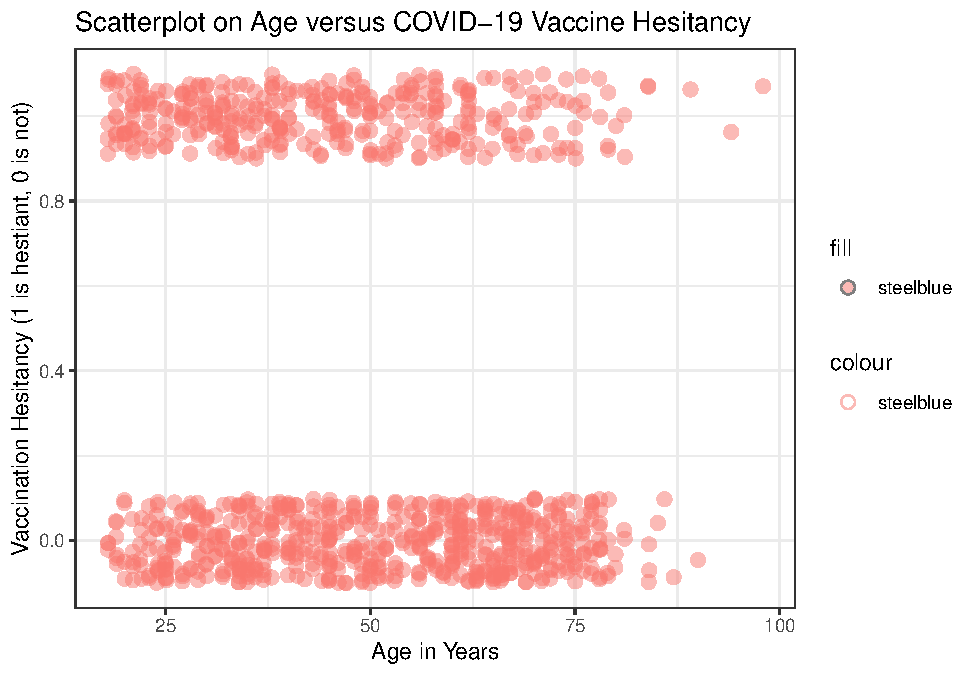
\includegraphics{Untitled_files/figure-latex/unnamed-chunk-4-1.pdf}

It is subtle, but notice that it seems like it seems like the older
someone is, there is a less likely hood that they are hesitant against
vaccine, as in our hitter scatterplot above, it seems to become more
dense in the 0 the older someone is, and also less dense in the 1 the
older someone is as well. However, perhaps a scatterplot is not the best
metric for truly finding substantiative evidence for what we want.

\hypertarget{bilbiography}{%
\section{Bilbiography}\label{bilbiography}}

Wagner, Abram. COVID-19 Vaccine Hesitancy Surveys. Ann Arbor, MI:
Inter-university Consortium for Political and Social Research
{[}distributor{]}, 2021-11-29. \url{https://doi.org/10.3886/E130422V3}

Akel et al.~Modification of a vaccine hesitancy scale for use in adult
vaccinations in the United States and China. Hum Vaccin Immunother.
2021. doi: 10.1080/21645515.2021.1884476

\end{document}
